\par{In this kernel we start taking as a base the previous kernel, but now we try to use private memory to reuse a complete row of
    matrix A, this should bring a performance improvement due to the use of on chip memories in every of these devices.}

\lstinputlisting[float,caption={Kernel making use of \emph{private memory}.},label={private_memory_kernel}, 
                style=customc]{/Users/clalanne/GitHubProjects/OpenCLNotes/src/code/private_memory.c}

\begin{figure}[!h]
    \centering
    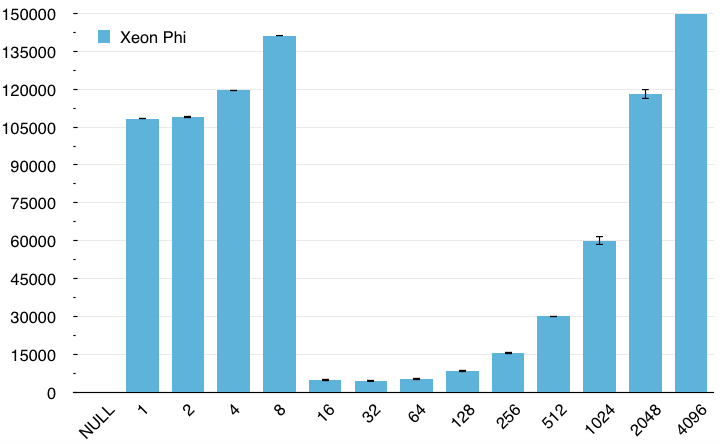
\includegraphics[width=0.49\textwidth]{figures/opt2_phi.png}
    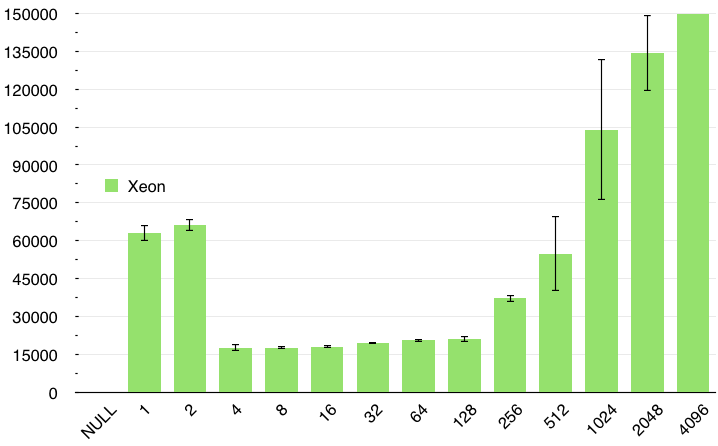
\includegraphics[width=0.49\textwidth]{figures/opt2_cpu.png}
    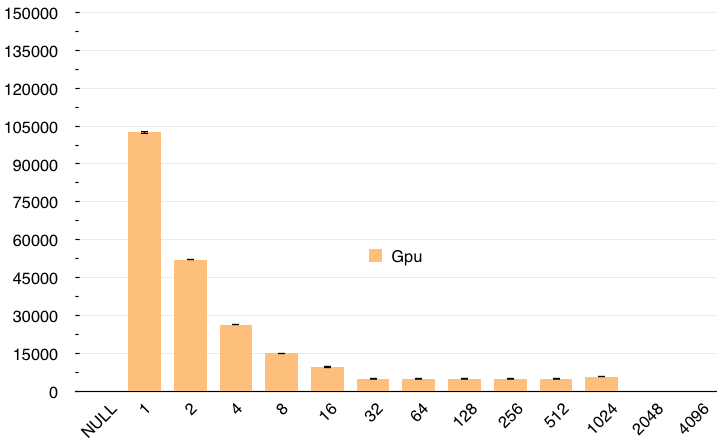
\includegraphics[width=0.49\textwidth]{figures/opt2_gpu.png}
    \caption{Row optimisation matrix multiplication in different architectures.}
    \label{Rows}
\end{figure}

\par{This kernel for Intel Xeon Phi and Xeon achieved a performance improvement in comparison with previous kernels as it can 
    be seen in figure \ref{Rows}. The use of OpenCL \emph{private memory} immediatelly increment the L1 hit ratio in both Intel
    Architectures(Xeon and Xeon Phi), also increments the vectorization intensity. Also we can see the effect of lost of parallelism
    due to the small amount of \emph{work groups} scheduled after a \emph{work group} dimension of 128.}

\par{In this case the most performant architecture for this kernel is the Intel Xeon Phi as it can be seen \ref{RowsComp}, 
    showing how sensible the Intel Xeon Phi in terms of memory optimisations.}

\par{\ref{RowsComp}}


\begin{figure}[!h]
    \centering
    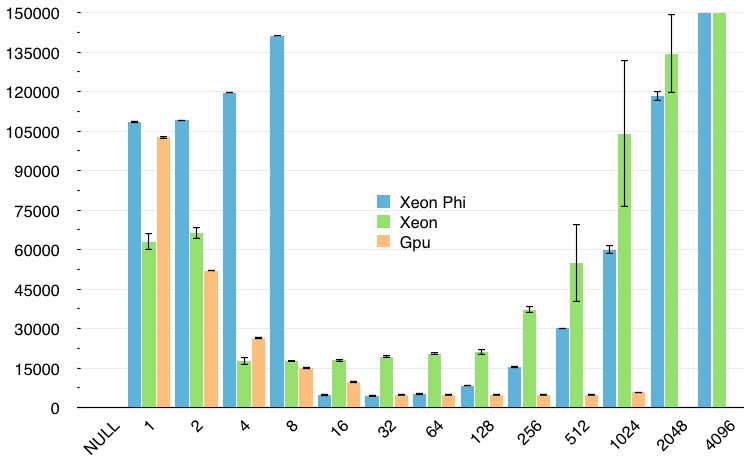
\includegraphics[width=0.6\textwidth]{figures/opt2_comp.png}
    \caption{Row optimisation matrix multiplication with more work in different architectures comparison.}
    \label{RowsComp}
\end{figure}

